\chapter{Advanced Strategies}\label{strat}

\section{Overview}\label{strat:overview}

Dakota's strategy capabilities were developed in order to provide a
control layer for managing multiple iterators and models. It was
driven by the observed need for ``meta-optimization'' and other high
level systems analysis procedures in real-world engineering design
problems. This capability allows the use of existing iterative
algorithm and computational model software components as building
blocks to accomplish more sophisticated studies, such as hybrid
minimization, multistart local minimization, or Pareto optimization.
Other strategy-like capabilities are enabled by the model recursion
capabilities described in Chapter~\ref{models}.  When these model
recursion specifications are sufficient to completely describe a
multi-iterator, multi-model solution approach, then a separate
strategy specification is not used (see Chapter~\ref{adv_models} for
examples).  In addition, some previous strategy capabilities (i.e.,
the surrogate-based minimization approaches descibed in
Chapter~\ref{sbm}) have migrated into the method specification to
allow their componentization and reuse elsewhere.  This trend will
continue in future releases so that only the most generic coordination
approaches will remain.

\section{Hybrid Minimization}\label{strat:hybrid}

In the hybrid minimization strategy (keyword: \texttt{hybrid}), a
sequence of minimization methods are applied to find an optimal design
point. The goal of this strategy is to exploit the strengths of
different minimization algorithms through different stages of the
minimization process. Global/local optimization hybrids (e.g., genetic
algorithms combined with nonlinear programming) are a common example
in which the desire for a global optimum is balanced with the need for
efficient navigation to a local optimum. An important related feature
is that the sequence of minimization algorithms can employ models of
varying fidelity. In the global/local case, for example, it would
often be advantageous to use a low-fidelity model in the global search
phase, followed by use of a more refined model in the local search
phase.

The specification for hybrid minimization involves a list of
method identifier strings, and each of the corresponding method
specifications has the responsibility for identifying the model
specification (which may in turn identify variables, interface, and
responses specifications) that each method will use (see the Dakota
Reference Manual~\cite{RefMan} and the example discussed below).
Currently, only the sequential hybrid approach is available. The
\texttt{embedded} and \texttt{collaborative} approaches are
not fully functional at this time.

In the \texttt{sequential} hybrid minimization approach, a sequence
of minimization methods is invoked in the order specified in the
Dakota input file. After each method completes execution, 
the best solution or solutions from that method are used as the
starting point(s) for the following method. 
The number of solutions transferred 
is defined by how many that method can generate and how many the 
user specifies with the individual method keyword \texttt{final\_solutions}. 
For example, currently only a few of the global optimization methods such as 
genetic algorithms (e.g. \texttt{moga} and \texttt{coliny\_ea}) and 
sampling methods return multiple solutions.  In this case, 
the specified number of solutions from the previous 
method will be used to initialize the subsequent method.  If the subsequent 
method cannot accept multiple input points (currently only a few methods 
such as the genetic algorithms in JEGA allow multiple input points), then 
multiple instances of the subsequent method are generated, each one 
initialized by one of the optimal solutions from the previous method. 
For example, if LHS sampling were run as the first method and 
the number of final solutions was 10 and the DOT conjugate gradient 
was the second method, there would be 10 instances of \texttt{dot\_frcg} 
started, each with a separate LHS sample solution as its initial point. 
Method switching is governed
by the separate convergence controls of each method; that is,
\emph{each method is allowed to run to its own internal definition of
completion without interference}. Individual method completion may be
determined by convergence criteria (e.g.,
\texttt{convergence\_tolerance}) or iteration limits (e.g.,
\texttt{max\_iterations}).  

%The \texttt{adaptive} option
%is similar, with the difference that the progress of each method is
%monitored and method switching is enforced according to
%externally-defined relative progress metrics.  

%The \texttt{embedded} approach is restricted to special tightly-coupled
%hybrid algorithms in which local searches are used periodically to
%accelerate a global search.  These hybrids do not contain a discrete
%method switch, but rather repeatedly apply a local algorithm within
%the context of the global algorithm.

Figure~\ref{strat:figure01} shows a Dakota input file that specifies
a sequential hybrid optimization strategy to solve the
``textbook'' optimization test problem. This input file is named
\texttt{dakota\_hybrid.in} in the \texttt{Dakota/test} directory.
The three optimization methods are identified using the
\texttt{method\_list} specification in the strategy section of the
input file. The identifier strings listed in the specification are
`\texttt{GA}' for genetic algorithm, `\texttt{PS}' for pattern search,
and `\texttt{NLP}' for nonlinear programming. Following the strategy
keyword block are the three corresponding method keyword blocks. Note
that each method has a tag following the \texttt{id\_method} keyword
that corresponds to one of the method names listed in the strategy
keyword block. By following the identifier tags from \texttt{method}
to \texttt{model} and from \texttt{model} to \texttt{variables},
\texttt{interface}, and \texttt{responses}, it is easy to see the
specification linkages for this problem. The GA optimizer runs first
and uses model `\texttt{M1}' which includes variables `\texttt{V1}',
interface `\texttt{I1}', and responses `\texttt{R1}'. 
Note that in the specification, \texttt{final\_solutions=1}, 
so only one (the best) solution is returned from the GA.  
However, it is possible to change this to \texttt{final\_solutions=5}
and get five solutions passed from the GA to the Pattern Search
(for example).  Once the GA is complete, the PS optimizer starts from the 
best GA result and again
uses model `\texttt{M1}'. Since both GA and PS are nongradient-based
optimization methods, there is no need for gradient or Hessian
information in the `\texttt{R1}' response keyword block. The NLP
optimizer runs last, using the best result from the PS method as its
starting point.  It uses model `\texttt{M2}' which includes the same
`\texttt{V1}' and `\texttt{I1}' keyword blocks, but uses the responses
keyword block `\texttt{R2}' since the full Newton optimizer used in
this example (\texttt{optpp\_newton}) needs analytic gradient and
Hessian data to perform its search.
\begin{figure}
  \centering
  \begin{bigbox}
    \begin{tiny}
      \verbatimtabinput[8]{dakota_hybrid.in}
    \end{tiny}
  \end{bigbox}
  \caption{Dakota input file for a hybrid optimization strategy.}
  \label{strat:figure01}
\end{figure}

\section{Multistart Local Minimization}\label{strat:multistart}

A simple, heuristic, global minimization technique is to use many
local minimization runs, each of which is started from a different
initial point in the parameter space. This is known as multistart
local minimization. This is an attractive strategy in situations where
multiple local optima are known or expected to exist in the parameter
space. However, there is no theoretical guarantee that the global
optimum will be found. This approach combines the efficiency of local
minimization methods with a user-specified global stratification
(using a specified \texttt{starting\_points} list, a number of
specified \texttt{random\_starts}, or both; see the Dakota Reference
Manual~\cite{RefMan} for additional specification details). Since
solutions for different starting points are independent, parallel
computing may be used to concurrently run the local minimizations.

An example input file for multistart local optimization on the
``quasi\_sine'' test function (see \texttt{quasi\_sine\_fcn.C} in
\texttt{Dakota/test}) is shown in Figure~\ref{strat:figure02}. The
strategy keyword block in the input file contains the keyword
\texttt{multi\_start}, along with the set of starting points (3 random 
and 5 listed) that will be used for the optimization runs. The other
keyword blocks in the input file are similar to what would be used in
a single optimization run.

\begin{figure}
  \centering
  \begin{bigbox}
    \begin{small}
      \verbatimtabinput[8]{dakota_multistart.in}
    \end{small}
  \end{bigbox}
  \caption{Dakota input file for a multistart local optimization strategy.}
  \label{strat:figure02}
\end{figure}

The \texttt{quasi\_sine} test function has multiple local minima, but
there is an overall trend in the function that tends toward the global
minimum at $(x1,x2)=(0.177,0.177)$. See~\cite{Giu00} for more
information on this test function. Figure~\ref{strat:figure03} shows
the results summary for the eight local optimizations performed. From
the five specified starting points and the 3 random starting points
(as identified by the \texttt{x1}, \texttt{x2} headers), the eight
local optima (as identified by the \texttt{x1*},
\texttt{x2*} headers) are all different and only one of the local
optimizations finds the global minimum.

\begin{figure}
\centering
\begin{bigbox}
\begin{footnotesize}
\begin{verbatim}
<<<<< Results summary:
   set_id             x1             x2            x1*            x2*         obj_fn 
        1           -0.8           -0.8  -0.8543728666  -0.8543728666   0.5584096919 
        2           -0.8            0.8  -0.9998398719    0.177092822    0.291406596 
        3            0.8           -0.8    0.177092822  -0.9998398719    0.291406596 
        4            0.8            0.8   0.1770928217   0.1770928217   0.0602471946 
        5              0              0  0.03572926375  0.03572926375  0.08730499239 
        6  -0.7767971993  0.01810943539  -0.7024118387  0.03572951143   0.3165522387 
        7  -0.3291571008  -0.7697378755   0.3167607374  -0.4009188363   0.2471403213 
        8   0.8704730469   0.7720679005    0.177092899   0.3167611757  0.08256082751 
\end{verbatim}
\end{footnotesize}
\end{bigbox}
\caption{Dakota results summary for a multistart local optimization strategy.}
\label{strat:figure03}
\end{figure}

\section{Pareto Optimization}\label{strat:pareto}

The Pareto optimization strategy (keyword: \texttt{pareto\_set}) is
one of three multiobjective optimization capabilities discussed in
Section~\ref{opt:additional:multiobjective}. In the Pareto
optimization strategy, multiple sets of multiobjective weightings are
evaluated. The user can specify these weighting sets in the strategy
keyword block using a \texttt{multi\_objective\_weight\_sets} list, a
number of \texttt{random\_weight\_sets}, or both (see the Dakota
Reference Manual~\cite{RefMan} for additional specification details).
Figure~\ref{strat:figure04} shows the input commands from the file
\texttt{dakota\_pareto.in} in the \texttt{Dakota/test} directory.

Dakota performs one multiobjective optimization problem for each set
of multiobjective weights. The collection of computed optimal
solutions form a Pareto set, which can be useful in making trade-off
decisions in engineering design. Since solutions for different
multiobjective weights are independent, parallel computing may be used
to concurrently execute the multiobjective optimization problems.

Figure~\ref{strat:figure05} shows the results summary for the
Pareto-set optimization strategy. For the four multiobjective
weighting sets (as identified by the \texttt{w1}, \texttt{w2},
\texttt{w3} headers), the local optima (as identified by the
\texttt{x1}, \texttt{x2} headers) are all different and correspond to
individual objective function values of ($f_1,f_2,f_3$) =
(0.0,0.5,0.5), (13.1,-1.2,8.16), (532.,33.6,-2.9), and (0.125,0.0,0.0)
(note: the composite objective function is tabulated under the
\texttt{obj\_fn} header).  The first three solutions reflect exclusive
optimization of each of the individual objective functions in turn,
whereas the final solution reflects a balanced weighting and the
lowest sum of the three objectives.  Plotting these ($f_1,f_2,f_3$)
triplets on a 3-dimensional plot results in a Pareto surface (not
shown), which is useful for visualizing the trade-offs in the
competing objectives.

\begin{figure}
  \centering
  \begin{bigbox}
    \begin{small}
      \verbatimtabinput[8]{dakota_pareto.in}
    \end{small}
  \end{bigbox}
  \caption{Dakota input file for the Pareto optimization strategy.}
  \label{strat:figure04}
\end{figure}

\begin{figure}
\centering
\begin{bigbox}
\begin{scriptsize}
\begin{verbatim}
<<<<< Results summary:
   set_id             w1             w2             w3             x1             x2         obj_fn
        1              1              0              0   0.9996554048    0.997046351 7.612301561e-11
        2              0              1              0            0.5            2.9           -1.2
        3              0              0              1            5.8 1.12747589e-11           -2.9
        4          0.333          0.333          0.333            0.5   0.5000000041       0.041625
\end{verbatim}
\end{scriptsize}
\end{bigbox}
\caption{Dakota results summary for the Pareto-set optimization
  strategy.}
\label{strat:figure05}
\end{figure}

%\section{Mixed Integer Nonlinear Programming (MINLP)}\label{strat:minlp}

%\emph{For Dakota 5.2, branch and bound is currently inoperative due to 
%ongoing restructuring of PICO and its incorporation into COLINY.
%This will be supported again in future releases.}

%Many nonlinear optimization problems involve a combination of discrete
%and continuous variables. These are known as mixed integer nonlinear
%programming (MINLP) problems. A typical MINLP optimization problem is
%formulated as follows:

%\begin{eqnarray}
%  \hbox{minimize:} & & f(\mathbf{x,d})\nonumber\\
%  \hbox{subject to:} & & \mathbf{g}_{L} \leq \mathbf{g(x,d)}
%    \leq \mathbf{g}_{U}\nonumber\\
%  & & \mathbf{h(x,d)}=\mathbf{h}_{t}\label{strat:equation01}\\
%  & & \mathbf{x}_{L} \leq \mathbf{x} \leq \mathbf{x}_{U}\nonumber\\
%  & & \mathbf{d} \in \{-2,-1,0,1,2\}\nonumber
%\end{eqnarray}

%where $\mathbf{d}$ is a vector whose elements are integer values. In
%situations where the discrete variables can be temporarily relaxed
%(i.e., noncategorical discrete variables, see
%Section~\ref{variables:design:ddv}), the branch-and-bound
%algorithm can be applied. Categorical variables (e.g., true/false
%variables, feature counts, etc.) that are not relaxable cannot be used
%with the branch and bound strategy.  During the branch and bound
%process, the discrete variables are treated as continuous variables
%and the integrality conditions on these variables are incrementally
%enforced through a sequence of optimization subproblems.  By the end
%of this process, an optimal solution that is feasible with respect to
%the integrality conditions is computed.

%Dakota's branch and bound strategy (keyword:
%\texttt{branch\_and\_bound}) can solve optimization problems having
%either discrete or mixed continuous/discrete variables. This strategy
%uses the parallel branch-and-bound algorithm from the PICO software
%package~\cite{Eck97,Eck01} to generate a series of optimization
%subproblems (``branches''). These subproblems are solved as continuous
%variable problems using any of Dakota's nonlinear optimization
%algorithms (e.g., DOT, NPSOL). When a solution to a branch is feasible
%with respect to the integrality constraints, it provides an upper
%bound on the optimal objective function, which can be used to prune
%branches with higher objective functions that are not yet
%feasible. Since solutions for different branches are independent,
%parallel computing may be used to concurrently execute the
%optimization subproblems.

%PICO, by itself, targets the solution of mixed integer linear
%programming (MILP) problems, and through coupling with Dakota's
%nonlinear optimizers, is extended to solution of MINLP problems. In
%the case of MILP problems, the upper bound obtained with a feasible
%solution is an exact bound and the branch and bound process is
%provably convergent to the global minimum. For nonlinear problems
%which may exhibit nonconvexity or multimodality, the process is
%heuristic in general, since there may be good solutions that are
%missed during the solution of a particular branch. However, the
%process still computes a series of locally optimal solutions, and is
%therefore a natural extension of the results from local optimization
%techniques for continuous domains. Only with rigorous global
%optimization of each branch can a global minimum be guaranteed when
%performing branch and bound on nonlinear problems of unknown
%structure.

%In cases where there are only a few discrete variables and when the
%discrete values are drawn from a small set, then it may be reasonable
%to perform a separate optimization problem for all of the possible
%combinations of the discrete variables. However, this brute force
%approach becomes computationally intractable if these conditions are
%not met. The branch-and-bound algorithm will generally require
%solution of fewer subproblems than the brute force method, although it
%will still be significantly more expensive than solving a purely
%continuous design problem.

%\subsection{Example MINLP Problem}\label{strat:minlp:example}

%As an example, consider the following MINLP problem~\cite{Eld99}:

%\begin{eqnarray}
%  \hbox{minimize:} & &
%  f(\mathbf{x})=\sum_{i=1}^{6}(x_{i}-1.4)^{4}\nonumber\\
%  & & g_{1}=x_{1}^{2}-\frac{x_{2}}{2} \leq 0\nonumber\\
%  & & g_{2}=x_{2}^{2}-\frac{x_{1}}{2} \leq 0\label{strat:equation02}\\
%  & & -10 \leq x_{1},x_{2},x_{3},x_{4} \leq 10\nonumber\\
%  & & x_{5},x_{6} \in \{0,1,2,3,4\}\nonumber
%\end{eqnarray}

%This problem is a variant of the textbook test problem described in
%Section~\ref{additional:textbook}. In addition to the introduction of
%two integer variables, a modified value of $1.4$ is used inside the
%quartic sum to render the continuous solution a non-integral solution.
%Figure~\ref{strat:figure06} shows a Dakota input file for solving this
%problem. This input file is named \texttt{dakota\_bandb.in} in the
%\texttt{Dakota/test} directory. Note the specification for the
%discrete variables, where lower and upper bounds are given. The
%discrete variables can take on any integer value within these bounds.

%\begin{figure}
%  \centering
%  \begin{bigbox}
%    \begin{small}
%      \verbatimtabinput[8]{dakota_bandb.in}
%    \end{small}
%  \end{bigbox}
%  \caption{Dakota input file for the branch-and-bound strategy for
%    solving MINLP optimization problems.}
%  \label{strat:figure06}
%\end{figure}

%Figure~\ref{strat:figure07} shows the sequence of branches generated
%for this problem.  The first optimization subproblem relaxes the
%integrality constraint on parameters $x_{5}$ and $x_{6}$, so that $0
%\leq x_{5} \leq 4$ and $0 \leq x_{6} \leq 4$. The values for $x_{5}$
%and $x_{6}$ at the solution to this first subproblem are
%$x_{5}=x_{6}=1.4$.  Since $x_{5}$ and $x_{6}$ must be integers, the
%next step in the solution process ``branches'' on parameter $x_{5}$ to
%create two new optimization subproblems; one with $0 \leq x_{5} \leq
%1$ and the other with $2 \leq x_{5} \leq 4$.  Note that, at this first
%branching, the bounds on $x_{6}$ are still $0 \leq x_{6} \leq 4$.
%Next, the two new optimization subproblems are solved.  Since they are
%independent, they can be performed in parallel.  The branch-and-bound
%process continues, operating on both $x_{5}$ and $x_{6}$ , until a
%optimization subproblem is solved where $x_{5}$ and $x_{6}$ are
%integer-valued. At the solution to this problem, the optimal values
%for $x_{5}$ and $x_{6}$ are $x_{5}=x_{6}=1$.

%\begin{figure}
%  \centering
%  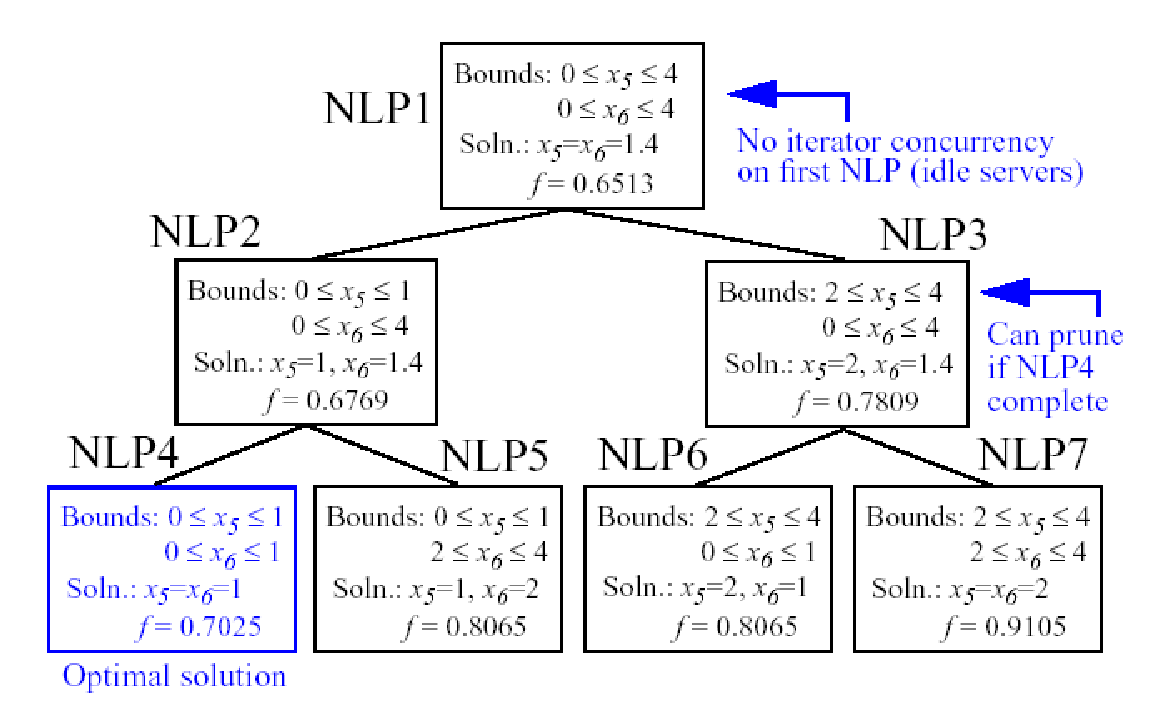
\includegraphics[scale=0.75]{images/branch_history}
%  \caption{Branching history for example MINLP optimization problem.}
%  \label{strat:figure07}
%\end{figure}

%In this example problem, the branch-and-bound algorithm executes as
%few as five and no more than seven optimization subproblems to reach
%the solution. For comparison, the brute force approach would require
%25 optimization problems to be solved (i.e., five possible values for
%each of $x_{5}$ and $x_{6}$ ).

%In the example given above, the discrete variables are integer-valued.
%In some cases, the discrete variables may be real-valued, such as $x
%\in \{0.0,0.5,1.0,1.5,2.0\}$.  The branch-and-bound algorithm is
%restricted to work with integer values. Therefore, it is up to the
%user to perform a transformation between the discrete integer values
%from Dakota and the discrete real values that are passed to the
%simulation code (see Section~\ref{variables:design:ddv}).  When
%integrality is not being relaxed, a common mapping is to use the
%integer value from Dakota as the index into a vector of discrete real
%values.  However, when integrality is relaxed, additional logic for
%interpolating between the discrete real values is needed.
% Note: it should be straightforward to extend MINLP to support
% general discrete variables, if PICO would support it.  Does this
% come up in MILP for logistics, etc.?
